\documentclass[12pt, a4paper, oneside]{book}

%\usepackage[utf8]{inputenc}
\usepackage{amsmath}
\usepackage{amsfonts}
\usepackage{amssymb}
\usepackage{graphicx}
\usepackage[left=1.5cm, right=5cm, bottom = 1cm, top = 2cm, headheight=16pt,
headsep = 0.5cm, foot = 16pt, footskip = 0.5cm]{geometry}
\setlength{\marginparwidth}{4.5cm}
\usepackage{marginnote}

\usepackage{fontspec}
\setmainfont{Charis SIL}
\usepackage{setspace}
\setstretch{1.1}
\usepackage[french]{babel}
\usepackage[babel=true]{csquotes}

\usepackage{soul}
\usepackage{mdframed}

\usepackage{xargs} % Use more than one optional parameter in a new commands
\usepackage[dvipsnames]{xcolor}


\usepackage{float}
\usepackage{caption}
\captionsetup[figure]{belowskip=-0.5cm}
\captionsetup[lstlisting]{belowskip=-0.25cm}
%\captionsetup[table]{position=above, aboveskip=0pt, belowskip=10pt}
\usepackage{rotating}
\usepackage{rotfloat}

\usepackage{fancyhdr}
\pagestyle{fancy}

\renewcommand{\headrulewidth}{0.5pt}
\renewcommand{\footrulewidth}{0pt}
\fancyhead[L]{Chapitre \thechapter}
\fancyhead[C]{}
\fancyhead[R]{\rightmark}

\usepackage{epigraph}

\newcounter{savefootnote}
\renewcommand{\thempfootnote}{\arabic{footnote}}%

\usepackage{enumitem}

\usepackage[hyperfootnotes=false]{hyperref}
\hypersetup{pdftitle={Robin Cura - Thèse}}
\usepackage[noabbrev, nameinlink]{cleveref}

\usepackage{longtable}
\usepackage{array}

\usepackage{fontawesome}
\usepackage{wrapfig}
\usepackage[style=authoryear-comp,
hyperref,
backend=bibtex,
isbn=false,
doi=true,
url=true,
date=year,
sortcites=false,  % Ne pas changer l'ordre des citations multiples
sorting=nyt % Citations dans biblio : NameYearTitle
]{biblatex}


%%%% Styles chapitres %%%%
\usepackage[Bjornstrup]{fncychap}
\ChTitleVar{\raggedright\LARGE\sffamily\bfseries}


%\usepackage{natbib}

\usepackage[thinlines]{easytable}
\usepackage{makecell}
\usepackage{diagbox}

\renewcommand\theadalign{bc}
\renewcommand\theadfont{\bfseries}
\renewcommand\theadgape{\Gape[4pt]}
\renewcommand\cellgape{\Gape[4pt]}

\usepackage[french, tight]{minitoc}
\dominitoc

\usepackage{listings} % Code
\lstset{
	basicstyle=\ttfamily,
	frame=single
}
%\usepackage{minted}
\renewcommand\lstlistingname{Code}
\renewcommand\lstlistlistingname{Code}
\crefformat{lstlisting}{code~#2#1#3}
\Crefformat{lstlisting}{Code~#2#1#3}

\usepackage[lofdepth,lotdepth]{subfig}
\usepackage{sparklines}

% ------------------------------------- %
% ---------- COMMANDES PERSO ---------- %
% ------------------------------------- %
% ######### TABLES AVEC FIGURES #########
\newcolumntype{M}[1]{>{\centering\arraybackslash}m{#1}}
\newcolumntype{N}{@{}m{0pt}@{}}
\usepackage{tikz}
\usetikzlibrary{calc,shapes,arrows}
\newcommand{\tikzmark}[1]{%
	\tikz[overlay,remember picture] \node (#1) {};}
% ############# SCHEMAS TIKZ ###########
\usepackage{tikz}
\usetikzlibrary{shapes,arrows.meta, shapes.geometric, positioning, patterns}
\usepackage{dashbox}

%%% TABLES
\usepackage{verbatim}
\usepackage{makecell}
\usepackage{multirow}

\usepackage{upgreek}

\setcounter{secnumdepth}{6}
\crefname{paragraph}{paragraphe}{paragraphes}
\Crefname{paragraph}{Paragraphe}{Paragraphes}

\makeatletter
\DeclareRobustCommand{\cnameref}[1]{%
%	\namecref{#1}
	\nameref{#1}%
}%
\DeclareRobustCommand{\Cnameref}[1]{%
	\nameCref{#1} \nameref{#1}%
}

% ###### CREATION D'ENCADRES ###### %

% Encadré pris dans la thèse de Seb Rey
\usepackage[most]{tcolorbox}
\newtcbtheorem[number within=chapter]{encadre}{Encadré}{
	outer arc=0pt,
	arc=0pt,
	breakable,
	enhanced,
	colback=white,
	colframe=black,
	colbacktitle=white,
	titlerule=0pt,
	fonttitle=\normalcolor\itshape}{enc}

\crefformat{tcb@cnt@encadre}{encadré~#2#1#3}
\Crefformat{tcb@cnt@encadre}{Encadré~#2#1#3}

% ###### COMMENTAIRES ###### %


% Surlignement texte (1) + commentaire en marge (2)

\DeclareRobustCommand{\hlorange}[1]{{\sethlcolor{Dandelion}\hl{#1}}}
\DeclareRobustCommand{\hlcyan}[1]{{\sethlcolor{Cyan}\hl{#1}}}

\newcommandx{\toChange}[2]{%
	\colorbox{Dandelion}{#1}\marginnote{\small\hlorange{#2}}%
}

\newcommandx{\Lena}[2]{%
	\colorbox{Cyan}{#1}\marginnote{\small\hlcyan{Lena:\\ #2}}%
}

% Highlight
\newcommandx{\fixref}[1]{\hl{#1}}

% ToDoBox
\newcommandx{\todobox}[2][1=]{%
	~\\	\colorbox{pink}{\parbox{0.9\textwidth}{%
		\vskip5pt
		\leftskip5pt\rightskip5pt
		#2
		\vskip5pt
	}~\\
}
}

% ######### TITRE #########
\usepackage{titling}
\title{Accompagner la modélisation des systèmes de peuplement par l’exploration interactive de données spatio-temporelles}
\author{Robin Cura}
\date{\vspace{-5ex}}
\makeatletter
\newcommand*{\toccontents}{\@starttoc{toc}}
\makeatother




\newskip\bigskipamount   \bigskipamount =20pt plus 4pt minus 4pt
\setlength{\parskip}{0.75em}
\setlength{\parindent}{2em}

\usepackage{titlesec} % Pose problème avec les headers
% Corrigé avec ce code, à mettre pour chaque section
%\let\orisectionmark\sectionmark
%\renewcommand\sectionmark[1]{}%
%\section[Titre TOC]{Titre dans texte}
%\orisectionmark{Titre header}
%\let\sectionmark\orisectionmark

\titlespacing\section{0pt}{16pt plus 4pt minus 2pt}{0pt plus 2pt minus 2pt}
\titlespacing\subsection{0pt}{11pt plus 4pt minus 2pt}{0pt plus 2pt minus 2pt}
\titlespacing\subsubsection{0pt}{11pt plus 4pt minus 2pt}{0pt plus 2pt minus 2pt}
\titlespacing\paragraph{2em}{6pt plus 2pt minus 2pt}{8pt plus 0pt minus 0pt}



% ######### PLAN DETAILLE #########
% Make a TOC without line number when calling \tableofcontents
%\let\Contentsline\contentsline
%\renewcommand\contentsline[3]{\Contentsline{#1}{#2}{}}
\usepackage{pbox}
\usepackage{array}% http://ctan.org/pkg/array



% ###### AVANT-PROPOS CHAP2 ######
\usepackage{multicol}


% ######## Plusieurs ndbp renvoyant à la même ######
\usepackage{footmisc}
% # Et on met un asterisque à la place
\newcommand{\astfootnote}[1]{
	\let\oldthefootnote=\thefootnote
	\setcounter{footnote}{0}
	\renewcommand{\thefootnote}{\fnsymbol{footnote}}
	\hspace*{-.45cm}\footnote{#1}\unskip
	\let\thefootnote=\oldthefootnote
}

% ############ CITATIONS #############
% Citer juste le prénom + nom d'une référence
\newrobustcmd*{\citeauteur}{\AtNextCite{\DeclareNameAlias{labelname}{first-last}}\citeauthor}
% \citeauteur{ref}


\begin{document}
\setcounter{part}{0}
\setcounter{chapter}{2}
%\part{Accompagner la modélisation d'une transformation dans le système de peuplement de l'Europe Médiévale}

\chapter{Paramétrer un modèle en situation d'interdisciplinarité}

Le modèle présenté dans le chapitre précédent est un \og état\fg{}, c'est-à-dire que les mécanismes, paramètres et les valeurs de ceux-ci correspondent à un instantané, potentiellement amené à évoluer.
Dans ce chapitre, nous nous attacherons à présenter le travail de paramétrage réalisé jusqu'ici, ayant abouti à la version du modèle tel que décrit auparavant.
Par paramétrage, et avant d'en spécifier le sens, nous entendons ici le processus visant à doter le modèle de paramètres (empiriques, \unsurec{mesurables}{trouver un terme} et techniques) lui permettant de mieux convenir aux objectifs fixés, soient-ils en terme de comportements attendus ou d'objectifs quantitatifs.

\section{Paramétrer ? Quoi et quand ?}

Le plus souvent (\fixref{ref Seb, Clem...}), une fois le modèle construit, le modélisateur s'attache à son paramétrage, en cherchant pour chaque paramètre la ou les valeurs qui permettront au modèle de s'approcher des données empiriques devant être reproduites.
Cette étape, que l'on nomme généralement calibration, peut se faire de manière manuelle, par approximations successives (\fixref{C. Cottineau et/ou S. Rey, d'après Hermann}), par semi-automatisme, par exemple en effectuant des analyses de sensibilité (\fixref{C. Schmitt, J. Hirtzel}), ou encore de manière entièrement automatique (\fixref{C. Schmitt, S. Rey, C. Cottineau avec PSE}).
L'approche souvent défendue, notamment dans les travaux les plus récents (\fixref{Rimbault?}), voudrait que cette étape soit obligatoire pour toute modélisation, permettant par une exploration systématique de comprendre l'entièreté du comportement d'un modèle, et d'en faire dès lors un outil complètement maitrisé rendant possible l'établissement d'une loi.

Dans notre travail, nous souhaitons revenir sur cette vision de la modélisation, en particulier en ce que nous considérons que cette pratique de recherches de valeurs optimales est un exercice qui devrait s'effectuer tout au long de la construction du modèle, de manière plus itérative que conclusive.


\subsection{Qu'est-ce que le(s) paramétrage(s) ?}

\subsubsection{Définition}

Le terme recouvre deux sens différents, ont la distinction peut se faire selon qu'on l'utilise pour définir un processus ou pour caractériser une configuration.
Dans ce deuxième cas, le paramétrage désigne un ensemble de valeurs de paramètres, par exemple quand on mentionne un paramétrage par défaut, ou un paramétrage optimal.
Pour ne pas risquer de contre-sens, nous préférerons le terme de configuration de paramètres.
Ici, nous emploierons plutôt le premier cas, définissant dès lors le paramétrage comme le processus, manuel ou automatique, visant à constituer cette configuration de paramètres.

On tend à distinguer le paramétrage -- presque hygiénique -- de la calibration, processus systématique qui inscrirait le modèle comme un outil scientifique et incontestable.
Nous choisissons ici de confondre ces approches, non pas en considérant le paramétrage comme un outil d'évaluation du modèle, mais comme une composante inhérente à la construction d'un modèle, quelque soient les formes et les temporalités que le paramétrage adopte.
Le paramétrage est en effet une pratique utile dans la construction du modèle, car les résultats auxquels il aboutit, c'est-à-dire les valeurs de paramètres qui semblent mieux adaptés, renseignent aussi bien sur les biais des mécanismes adoptés que sur leur efficacité réelle.
Par exemple, quand, après avoir ajouté un mécanisme, on se rend compte que des variations dans les valeurs de paramètres ne changent pas réellement les sorties du modèle, cela peut être l'occasion de repenser le mécanisme dans son ensemble, ou plus souvent, la manière dont le paramètre est mobilisé dans ce mécanisme.

\subsubsection{Un modèle, des modèles}

\fixref{Cottineau, Reuillon et Rey} ont montré qu'on construisait plus souvent des familles de modèles que des modèles uniques.
Ces auteurs plaident pour une construction modulaire de modèles, chacun des mécanismes et complexifications devant être autonomes afin de pouvoir les assembler en autant de combinaisons que nécessaire à une exploration d'ensemble de leurs interactions.

Nous reprendrons de leur discours une vision moins ambitieuse, en considérant (\unsurec{ref Rey}{à chercher il en parlait à sa soutenance je crois}) simplement qu'en fait d'un modèle, la modélisation passe par plusieurs modèles, chacun se devant dès lors d'être adapté par un paramétrage dédié.

Pour illustrer ce propos, on peut prendre l'exemple d'une modification qui a eu lieu sur notre modèle au cours de son développement. On considérait jusque là que pour prendre en compte la population rurale (hors Tours donc), $1000$ foyers paysans donnaient une bonne idée de la situation en 800 pour l'espace considéré.
Lors d'une réunion, les thématiciens se sont rendus compte que ce nombre sous-estimait très largement la population réelle, et qu'il valait mieux passer ce paramètre à $4000$ foyers paysans.
Les autres paramètres, fixés en bonne partie empiriquement, n'avaient visiblement aucune raison d'évoluer du fait de ce changement. Les mécanismes  et effets de seuil étaient en effet conçus de manière à être relatifs aux masses manipulées, et le changement attendu était une augmentation linéaire des indicateurs de sortie.

Dans les faits, cette légère modification a entraîné une obligation de repenser la quasi-totalité des autres paramètres et d'ajuster une bonne part des règles. 
La concentration des foyers paysans était en effet bien trop rapide avec autant d'individus, et le modèle convergeait en quelques pas de temps vers une configuration presque statique et très concentrée.
Tous les mécanismes de régulation de ce comportement étaient dès lors rendus ineptes, et il a fallu changer en profondeur la manière dont chaque paramètre et mécanisme interagissait avec les autres.
C'est un changement majeur, que l'on peut constater dans la figure~\ref{fig:comits-periodes} (1ère modification de la période B), ayant donc entraîné des adaptations de tous les plans du modèle (paramètres en B, mécanismes en C).
La première version avait été paramétré aussi correctement que possible, mais ce paramétrage était entièrement à refaire avec la nouvelle version (modifications de la période B, \cref{fig:comits-periodes}).
On pourrait dès lors différencier le modèle pré-existant et celui qui a suivi ce changement, et les considérer comme deux modèles puisque réagissant de manière extrêmement différente.

\begin{figure}[!h]
	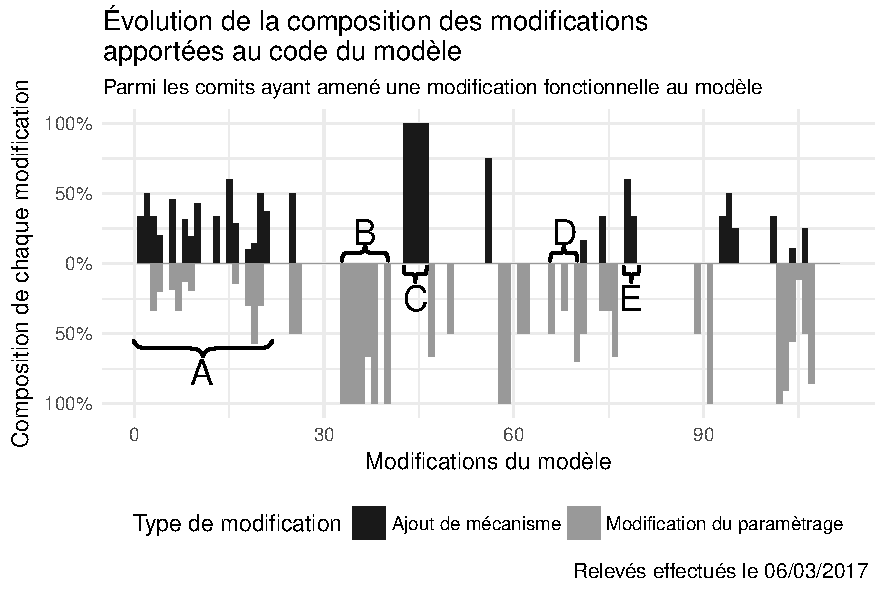
\includegraphics[width = \linewidth]{img/plotComits.pdf}
	\caption{Temporalité du paramétrage du modèle.\\
	Chaque \og enregistrement\fg{} (\textit{comit}) correspond à une sauvegarde du modèle, contenant un ou plusieurs changements. On a ici rapporté le nombre de changements de chaque type au nombre total de changements de chaque \textit{comit} afin de démarquer des types de \textit{comits}.}
	\label{fig:comits-periodes}
\end{figure}

Cet exemple renforce le caractère nécessaire du paramétrage, et qui plus est, de la continuité de cette étape, qui ne peut être pensée que comme une calibration finale d'un modèle abouti, auquel on ne peut en fait parvenir que par des paramétrages réguliers de modèles successifs moins aboutis.

\subsubsection{Désambiguïsation}

De nombreux termes sont utilisés dans la littérature, souvent sans réelle distinction, pour désigner cette opération qui consister à choisir un jeu de paramètres pour un modèle. Pêle-mêle, on y retrouve le paramétrage, la validation, l'évaluation ou encore la calibration. Nous définissons dans l'\cref{enc:termes-calibration} le sens donné à chacun de ces termes dans le cadre de ce manuscrit.

\begin{encadre}{Calibration, évaluation, validation\ldots\label{enc:termes-calibration}}
	\begin{description}[style=nextline]	
		\item[Calibration] On réserve souvent, et nous nous y tiendrons, ce terme à la dernière étape dans l'aboutissement d'un modèle.
		Une fois les mécanismes fixés et des objectifs définis, on peut procéder à la calibration, c'est-à-dire à une exploration de l'espace des paramètres ayant pour but de stabiliser les paramètres afin de se rapprocher autant que possible de ces objectifs.
		Cette étape, quelques soient les moyens employés, s'approche de la résolution utilisée dans le cadre de systèmes d'équations.
		Le contexte des systèmes complexes, et donc d'une non-linéarité des effets des paramètres, rend toutefois difficile l'obtention d'une unique configuration de paramètres optimale, et la calibration aboutit donc souvent à un ensemble de configurations possibles, constituant par exemple un optimum de Pareto (\fixref{Trouver ref}).
		
		\item[Évaluation] On emploie majoritairement ce mot pour décrire les méthodes permettant de comprendre le comportement du modèle et sa réaction aux différents paramètres.
		Là où la calibration cherche une configuration de paramètres optimale, l'évaluation tend surtout à caractériser la stabilité du modèle face à l'aléa ou a des configurations exceptionnelles.
		On vise ainsi à s'assurer que le modèle reproduise les faits stylisés voulus quelque soient son réglage, ou au moins à quantifier les intervalles de paramètres qui y satisfont.
		
		\item[Validation] La validation (refs Seb) tire son origine de sciences plus nomothétiques, et correspond donc à la démonstration qu'un modèle reproduit correctement ce qu'il représente. Au delà de l'évaluation, le terme amène une logique de preuve formelle que le modèle réagit bien ainsi et pas autrement quelque soient les conditions d'exécution. Cette démonstration formelle peut être effectuée sur des modèles à faible nombre de paramètres et mécanismes, mais le terme n'est jamais (à vérifier) employé dès lors que les modèles se complexifient.
	\end{description}
\end{encadre}


\subsection{Quand paramètre-t-on un modèle ?}

Le paramétrage du modèle n'est pas une étape unique, qui se déroulerait une fois le modèle construit, d'une manière complètement automatisable, permettant l'aboutissement d'un modèle désormais finalisé.
Au lieu de cela, le paramétrage se fait par étapes successives, chaque modification des hypothèses, des mécanismes, des objectifs ou encore des paramètres amenant à une nouvelle phase de paramétrage.
Afin que les \ref{}comportements du modèle soient cohérents avec les attendus, il convient donc de paramétrer le modèle aussi souvent que possible, à chaque modification de chacune de ses parties.
Un premier paramétrage, souvent non mentionné, tient ainsi lieu lors de la construction en elle-même du modèle, et vise en particulier à doter les paramètres techniques \change{ref vers chap2 et encadré types de paramètres} de valeurs permettant aux autres paramètres de donner satisfaction avec des ordres de grandeur cohérents.

\subsubsection{Tout au long de la construction}

Comme le montre la \cref{fig:comits-periodes}, les étapes de paramétrage sont omniprésentes sur la durée de construction du modèle. On peut en effet y noter que les \textit{comits} du code portant sur des modifications de valeurs de paramètres sont très réguliers.
Au delà de la valeur illustrative de ce modèle particulier, c'est un comportement que l'on retrouve régulièrement sur les modèles dont l'évolution est documentée, ce que le recours de plus en plus fréquent à des outils de versionnement (git en particulier) encourage.

La régularité et le systématisme du paramétrage sont bénéfiques à la création d'un modèle en ce qu'ils impliquent une utilisation fréquente du modèle, et une utilisation plus poussée : le paramétrage implique de tester plusieurs valeurs, et donc d'executer le modèle de nombreuses fois, d'autant plus en prenant en compte les réplications nécessaires à la prise en compte de l'aléa d'un modèle.

Une analogie peut être faite avec un principe populaire dans le développement de logiciel libre, résumé par le mot d'ordre \og \textit{release early, release often}\fg{}\footnote{Mot d'ordre en particulier popularisé par Eric Raymond, l'un des \og évangélistes\fg{} du logiciel \textit{open-source}.}.
Selon ce principe, une publication régulière et rapide du code source d'un logiciel permet d'avoir un retour rapide de la communauté des utilisateurs, et ainsi de faire remonter d'éventuels \textit{bugs} et régressions bien plus rapidement que dans une voie plus classique.

Un modèle, dès qu'il devient suffisament complexe pour que les modifications n'apportent pas que des changements prévisibles, est souvent sujet à des \og effets de bord \fg{}, c'est-à-dire des comportements irrationnels spécifiques qui n'arrivent que dans certaines conditions particulières.
Comme dans n'importe quel logiciel informatique, les \textit{bugs} les plus compliqués à résoudre sont ceux dont on ne comprend pourquoi ou quand ils se déclenchent.
Les modèles réagissent de la même manière, provoquant de temps en temps des erreurs ou des comportements aberrants sans que l'on soit en mesure de les reproduire facilement. Un paramétrage régulier entraîne une plus forte probabilité de survenance de ces cas particuliers, et dès lors, une meilleure résistance des mécanismes.

\subsubsection{À chaque ajout ou changement de mécanisme}

De manière plus spécifique, et pour les mêmes raisons qu'évoquées auparavant, il est indispensable de réaliser un paramétrage à chaque fois que les mécanismes de mobilisation d'un paramètre changent.

Le paramétrage permet de s'assurer de la cohérence des mécanismes et paramètres les uns avec les autres.
Que le modèle soit construit par une seule personne ou par plusieurs, il est plus simple de corriger une erreur ou un comportement inattendu quand les modifications depuis le dernier état stable sont faibles plutôt que quand de nombreux changements ont été effectués.
En effet, la résolution d'erreurs nouvelles dans un modèle se résume souvent à activer et désactiver les ajouts, un par un, afin de trouver la modification responsable.
Dans un modèle complexe où les mécanismes et paramètres sont en partie interdépendants, quand plusieurs modifications sont effectuées, les petites erreurs et incompatibilités de chacune se combinent en des problèmes tout aussi complexes que les systèmes modélisés.
On gagne donc énormément de temps de correction du modèle en identifiant régulièrement les problèmes, ce qu'un paramétrage à chaque changement permet.

Le recours régulier à un paramétrage remplit ainsi exactement le même rôle que les \og bancs de test\fg{} de l'industrie, c'est-à-dire qu'il permet d'évaluer (cf. \cref{enc:termes-calibration}) un modèle à chacune des modifications, s'assurant donc de sa qualité tout au long et minimisant le risque d'erreurs et donc la durée des phases de paramétrages plus importants.

\subsubsection{Avant toute modification majeure du modèle}

Si le paramétrage a été régulier dans la construction du modèle, on note toutefois, dans la figure \ref{fig:comits-periodes}, que certaines phases (période B en particulier, mais aussi D) se caractérisent par une forte tâche de paramétrage avant une période de changement (C et E respectivement).
Cela correspond à une phase d'exploration plus poussée du modèle, en vue de le faire évoluer par la suite, par exemple en complexifiant les mécanismes à l'oeuvre pour le rendre plus conforme aux attentes.

Quand le paramétrage n'est pas bien exécuté avant ces changements, les mécanismes à adapter sont moins clairs et moins bien compris, et un travail plus important d'essai-erreur est requis, comme les premiers temps de la construction du modèle (période A) l'illustrent : faute de bonne compréhension du modèle, l'évolution est plus poussive, dans un aller-retour constant entre paramétrage et ajout/modification de mécanismes.

Ce principe s'inscrit dans les méthodes de développement qualifiées d'\og agiles\fg{}, qui insistent en particulier sur l'\changec{incrémentalité}{Je reprendrais ça en chap. 7, dans un encadré différenciant bien itératif/incrémental\\cf. \href{https://ravisr16.wordpress.com/2014/06/22/agile-development-environment/}{Agile Development Environment @ ravisr16}} de la construction : à chaque étape, aussi peu différente soit-elle de la précédente, le logiciel (ou le modèle ici) doit être fonctionnel, et on ne passe pas à une version suivante tant que ce n'est pas le cas.

\subsection{Comment paramétrer ?}


\subsubsection{Visual validation}

(Trouver ref dans thèse Clémentine, sans doute Hermann encore)

\subsubsection{Indicateurs}

\subsubsection{L'importance de la réplication}


\section{Premiers paramétrages}

	\subsection{Au fil de la construction}
	
		\subsubsection{Paramétrage technique}
		
		\subsubsection{Ajout de paramètres}
	
	\subsection{Paramétrer \textit{in situ}}
	
		\subsubsection{Paramétrage empirique}
		
		\subsubsection{Changements majeurs}

	\subsection{Première exploration systématique}
	
	
\section{Premiers résultats du paramétrage}

	\subsection{Tendances}

	\subsection{Variabilité}

\section{Comment traiter les sorties du/des modèle(s) ?}

	\subsection{Nombre de sorties}
	
	\subsection{Masse de sorties}


\end{document}

## Chapitre 3 : Paramétrer un modèle en situation d'interdisciplinarité
- Premier paramétrage du modèle (avec Samuel etc.)
- Calibration du modèle (avec CT)
- Premiers résultats (contenu chap 11 TMD)
- Quelle variabilité du modèle ? Pour quelles raisons (aléa init. vs aléa mécanique) ?
- Sorties graphiques, rapports, rapports ++
- Comment aller plus loin ?